\chapter {Description formelle de l'éditeur de composants métiers caractéristiques}

\section{Présentation de l'éditeur}
L'embryon de plateforme existant pour la méthode FORM/BCS a été développé en Java en utilisant le framework Eclipse EMF(Eclipse Modeling Framework). EMF est un environnement de modélisation et de génération de code qui facilite la construction d'outils et d'applications sur les modèles de données structurées. Il est basé sur l'Ingénierie Dirigée par les Modèles (IDM); l'approche de développement IDM consiste à séparer les spécifications fonctionnelles d'un système de son implémentation. Elle préconise pour ce faire de construire trois principaux modèles pour aboutir à la génération du code source 
\begin{itemize}
	\item CIM (Computational Independent Model) qui modélise les exigences fonctionnelles du système
	\item PIM (Platform Independent Model) ou encore modèle conceptuel qui est un modèle abstrait, indépendant de toute plateforme d'exécution 
	\item PSM (Platform Specific Model) qui est un modèle technologique de plus bas niveau dépendant de la plateforme d'exécution.
	\item Le code source est généré à partir de la PSM. 
	\end{itemize}
	
	La figure figure \ref{fig:MDA_process}
	
\begin{figure}[h!]
  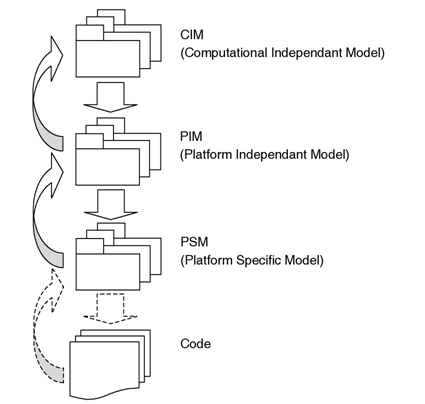
\includegraphics[scale=0.7]{images/mda_technology.png}
  \caption{Processus de Ingénierie Dirigée par les Modèles}
  \label{fig:MDA_process}
\end{figure}
	
	Ainsi, EMF génère du code source en transformant différents modèles. Il permet également de générer des éditeurs textuels ou graphique. Le point d'entrée est un modèle appelé Ecore, c'est le Méta-modèle d'EMF, il est indépendant de la plateforme d'execution car ne contient aucne information à propos des packages ou des classes Java. Ce dernier peut être spécifié en utilisant l'éditeur graphique qu'offre EMF ou en important des interfaces Java, un diagramme de classe UML ou un schéma XML. Le méta-modèle Ecore étant indépendant de toute plateforme d'exécution, pour générer du code Java, il faut spécifier un modèle de génération qui contient les informations de plateforme (packages, classes...): c'est le \textsl{genmodel}; il peut être généré automatiquement à partir du modèle Ecore. Associé à EMF, le plugin EMFTEXT permet de générer des éditeurs pour les DSL (Domain Specific Language) avec des fonctionnalités avancées telles que l'autocomplétion, la coloration du texte, la personnalisation de la syntaxe, le rapport instantané des erreurs etc. C'est ce plugin qui a été utilisé pour la réalisation de l'embryon de plateforme pour le projet REAL. 

\begin{figure}[h!]
  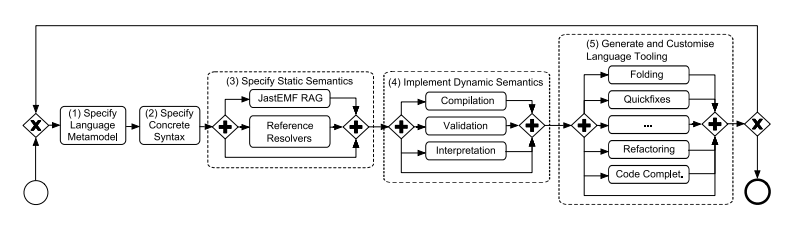
\includegraphics[scale=0.7]{images/EMFTEXT_process.png}
  \caption{Processus de développement d'un langage avec EMFTEXT}
  \label{fig:EMFTEXT_process}
\end{figure}

La génération d'un éditeur sophistiqué pour un nouveau langage necessite juste quelques étapes de spécification et de génération avec EMFTEXT comme le montre la figure \ref{fig:EMFTEXT_process}. Ces étapes sont les suivantes:
\begin{enumerate}
	\item spécifier le métamodèle Ecore
	\item spécifier la syntaxe concrète
	\item (optionnelle) spécifier la sémantique statique 
	\item (optionnelle) implémenter la sémantique dynamique 
	\item générer et (optionnellement) modifier l'éditeur, par exemple en personnalisant la complétion de code, la mise en valeur de la syntaxe etc.
\end{enumerate}

De ces étapes, seules les étapes (1) et (2) sont obligatoires ainsi que la génération du code de l'éditeur (étape 5). C'est par ces dernières que le plugin REAL a été généré. 
\subsection{Description non-formelle de l'embryon}
Le plugin généré a été baptisé REAL. Il se compose des différents éléments suivants:
\begin{enumerate}
	\item spécifier le métamodèle Ecore
	\item spécifier la syntaxe concrète
	\item (optionnelle) spécifier la sémantique statique 
	\item (optionnelle) implémenter la sémantique dynamique 
	\item générer et (optionnellement) modifier l'éditeur, par exemple en personnalisant la complétion de code, la mise en valeur de la syntaxe etc.
\end{enumerate}
\begin{figure}[h!]
  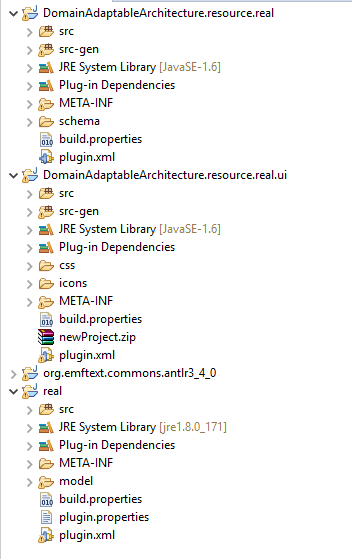
\includegraphics[scale=0.9]{images/real.png}
  \caption{Plugin REAL}
  \label{fig:plugin_real}
\end{figure}
\section{Description formelle}
1.Décrire les packages de REAL sous forme de composants(modules)
2.Montrer la communication entre ces modules
3.Parler des EXTENSIONS POINTS

